\subsection{Un peu de vocabulaire pour mieux se comprendre}
\begin{description}
  \item[Le HTML] est le langage utilisé pour écrire le contenu des pages web.
  \item[Le CSS] est un langage complémentaire au HTML. Il permet de
    décrire le style des éléments HTML comme leur taille, leur couleur et autres
    propriétés.
  \item[Les balises] permettent de décrire le contenu d'une page et
    s'organisent entre elles comme des dossiers imbriqués.
    Elles se présentent sous la forme suivante : \mintinline{xml}{<type_balise> </type_balise>}.
    Ici \mintinline{xml}{<type_balise>} ouvre la balise, et\mintinline{xml}{</type_balise>}
    la ferme.
  \item[Les attributs] Certaines balises peuvent avoir des attributs. Une
    balise « article » avec un attribut « couleur\_fond » ayant
    pour valeur « rouge » s’écrira de la façon suivante :
    \mintinline{xml}{<article couleur_fond="rouge"></article>}
\end{description}

\section{HTML de base}
Voici un petit exemple de code html :

\begin{minipage}{0.55\textwidth}
\begin{minted}{html}
<!DOCTYPE HTML>
<html>
    <head>
        <meta charset="utf-8">
        <title>
            Bienvenue à GCC !
        </title>
    </head>
    <body>
        GCC, c'est cool \o/
    </body>
</html>
\end{minted}
\end{minipage}
\begin{minipage}{0.45\textwidth}
\begin{minted}{html}
Indique que c'est du HTML
Début du code HTML
    Début des informations
        Pas important
        Début du titre
            Titre
        Fin du titre
    Fin des informations
    Début du contenu
        Contenu
    Fin du contenu
Fin du code HTML
\end{minted}
\end{minipage}\\

\section{Les balises}
\begin{description}
\item[\mintinline{xml}{<p>}] Permet d'afficher un paragraphe de texte.
\item[\mintinline{xml}{<br>}] Permet de mettre un retour à la ligne. Pas besoin
  de fermer cette balise !
\item[\mintinline{xml}{<h1>}, \mintinline{xml}{<h2>}, \mintinline{xml}{<h3>}] Les
  balises h nous permettent d’écrire des titres. Le chiffre indique l'importance
  du titre. Généralement, h1 est le titre de la page, h2 le sous-titre, etc…
\item[\mintinline{xml}{<img>}] Les balises img vont nous permettre d’insérer les
  photos sur notre page.
\item[\mintinline{xml}{<a href="https://prologin.org/">}] Permet de créer un
  lien vers un site internet.
\item[\mintinline{xml}{<div>}] N'affiche rien de spécial, mais vous permet du
  coup de faire des groupes de balises !
\end{description}

\subsection{Images}
Pour insérer des images il faut utiliser les balises \mintinline{xml}{<img>}.

Pour définir quelles images celles-ci vont afficher, il faut utiliser l’attribut
\textit{src}, avec pour valeur un chemin depuis la page actuelle vers l'image à
afficher.

\mintinline{html}{<img src="images/arbre.jpg" alt="C’est une photo d’un arbre"></img>}
À noter que pour permettre aux malvoyants de visiter votre site, il est
conseillé d’ajouter un attribut \textit{alt}, contenant une description de la photo.\\

Par exemple, dans le dossier suivant:\\

\dirtree{% ce commentaire est utile, pas touche
.1 \texttt{index.html}.
.2 \texttt{images}.
.3 \texttt{mon\_image.png}.
}
\hfill\\
Pour afficher \texttt{mon\_image.png} depuis \texttt{index.html}, on utilisera
le chemin:
\begin{center}
  \texttt{images/mon\_image.png}.
\end{center}
\hfill\\

\begin{exercise}
  Créez le document \texttt{index.html} contenant du texte et une image.
  Lancez la commande \texttt{firefox index.html} pour l'afficher ! Pour l'image,
  vous pouvez la télécharger sur internet ou lancer \texttt{gimp} et créer la
  vôtre.
\end{exercise}

\section{Du CSS, pour le plaisir des yeux}

Le CSS, c'est un langage qui permet de décrire comment doit apparaître le
contenu écrit en HTML.\\

En CSS, on écrit des règles qui s'appliquent à certains éléments :

\begin{alltt}
\colorbox{blue!30}{type_élément} \{
        \colorbox{green!30}{attribut}: \colorbox{red!30}{valeur};
        \colorbox{green!30}{attribut}: \colorbox{red!30}{valeur};
        ...
\}
\end{alltt}

\subsection{Insérer du CSS dans la page}

Pour insérer du CSS dans une page, on écrit notre code entre des balises
\mintinline{xml}{<style>}.

\subsection{Petite introduction}
Prenons par exemple le bout de code HTML suivant:

\begin{minted}{html}
<!DOCTYPE HTML>
<html>
    <head>
        <meta charset="utf-8">
        <title>
            Bienvenue à GCC !
        </title>
    </head>
    <body>
        <h1> Ceci est un titre ! </h1>
    </body>
</html>
\end{minted}

Si on veut donner au titre une couleur plus joyeuse que du noir, on peut
joindre le CSS suivant :

\begin{minted}{css}
h1 {
    color: blue;
}
\end{minted}

Le code devient ainsi :

\begin{minted}{html}
<!DOCTYPE HTML>
<html>
    <head>
        <meta charset="utf-8">
        <title>
            Bienvenue à GCC !
        </title>
        <style>
        h1 {
            color: blue;
        }
        </style>
    </head>
    <body>
        <h1> Ceci est un titre ! </h1>
    </body>
</html>
\end{minted}

\begin{exercise}
  Comparez les deux exemples.
\end{exercise}

Maintenant que vous connaissez la syntaxe, voyons quelques propriétés
intéressantes :

\begin{description}
\item [color] permet de changer la couleur d’un élément, on
  peut soit  indiquer le nom de couleur en anglais, soit en hexadécimal (
  \#RRGGBB ).
\item [background-color] même chose que pour \texttt{color}, pour
  l’arrière-plan d’un élément.
\item [background-image] permet de changer l’arrière-plan
  d’un élément par une image avec le valeur : url("chemin/vers/image.png").
\item [font-family] permet de changer la police d’un texte,
  par exemple\\ \mintinline{yaml}{font-family: Verdana}
\item [font-size] permet de changer la taille d’un texte,
  par exemple\\ \mintinline{html}{font-size: 26px}
\item [font-style] permet par exemple de mettre un texte en
  italique avec la valeur : italic.
\item [font-weight] permet de changer l’épaisseur d’un texte
  avec les valeurs :
  \begin{description}
    \item[lighter] moins épais
    \item[bold] gras
  \end{description}
\item [text-align] permet de changer l’alignement d’un texte
  avec les valeurs :
  \begin{description}
  \item[center] centré
  \item[justify] justifie le texte (aligne les fins de ligne en une colonne)
  \item[left] à gauche
  \item[right] à droite
  \end{description}
\item [text-decoration] permet d'ajouter certains effets à un
  texte avec les valeurs :
  \begin{description}
  \item[line-through] texte barré
  \item[overline] surligné
  \item[underline] souligné
  \end{description}
\item [text-transform] permet de changer la case d’un texte
  avec les valeurs :
  \begin{description}
  \item[capitalize] mettre seulement des  majuscule à chaque début de mot
  \item[lowercase] tout en minuscule
  \item[uppercase] tout en majuscule
  \end{description}
\item [margin] permet de changer les marges d’un élément avec
  une valeur en pixel ou avec la valeur \textit{auto} qui permet de centrer un
  élément (très très utile).
\item [padding] permet de laisser plus d’espace entre les
  éléments, sans les agrandir (prend une valeur en pixel).
\item [width] permet de spécifier la largeur de la page, soit
  en pixel (\mintinline{html}{16px} par exemple), soit en pourcentage (100\%
  par exemple).
\item [height] similaire à \mintinline{html}{width} mais pour la hauteur.
\end{description}

\subsection{Amélioration...}

Maintenant que vous maîtrisez le CSS à la perfection, il est temps de faire
vos preuves !

Votre objectif est de transformer ce que vous avez réalisé précédemment en
quelque chose de plus beau ! Vous pouvez vous inspirer du modèle ci-dessous :
\begin{center}
  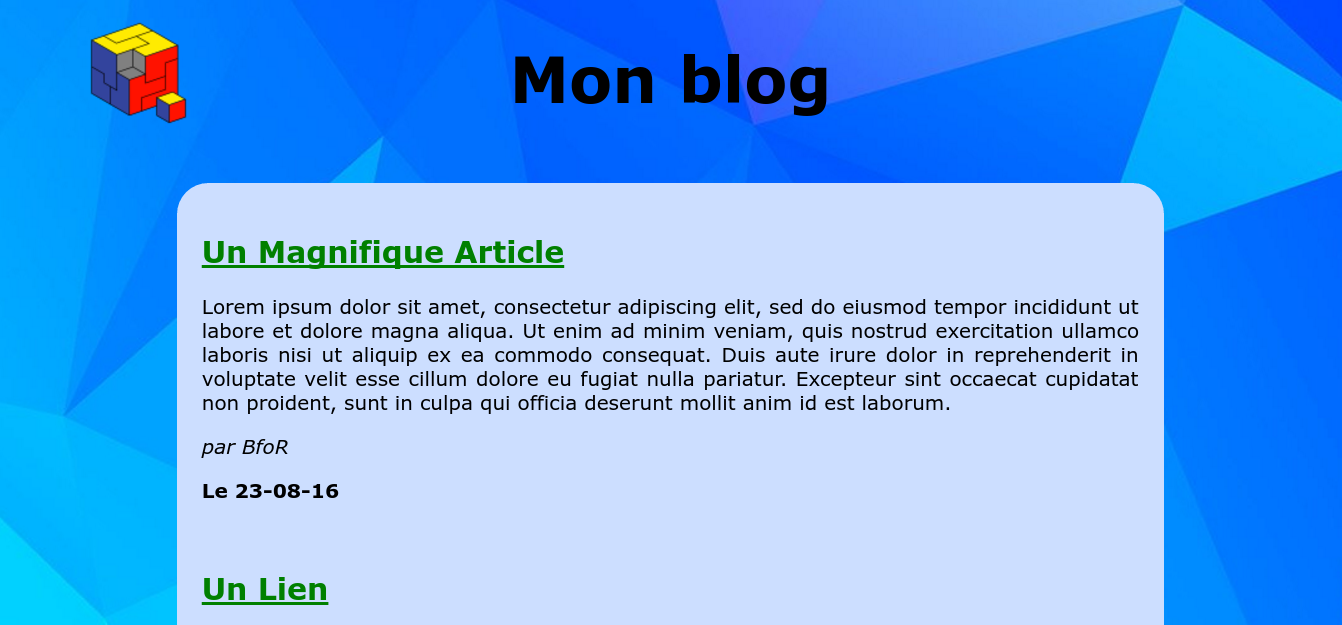
\includegraphics[width=0.8\textwidth]{img/image1.png}
\end{center}
\section{Soudainement, Python !}

Imaginez un instant:\\
Et si un programme Python de votre conception écrivait du code \texttt{html} à
votre place ?\\

Fou ? Pas tant que ça ! Regardez le programme suivant:

\begin{minted}{python}
# on dit à python qu'on veut pouvoir utiliser le
# groupe de fonctions « random »
import random

# pareil avec la fonction « Flask », du groupe « flask »
from flask import Flask

# La fonction Flask permet de créer un nouveau site
site = Flask("Mon Site")

citations = [
    "Je suis une olive",
    "Perdu",
    "On est vendredi !",
]

# les trois " servent à mettre du texte sur plusieurs lignes
début_réponse = """
<!DOCTYPE HTML>
<html>
    <head>
        <meta charset="utf-8">
        <title>
            Bienvenue à GCC !
        </title>
    </head>
    <body>
"""

fin_réponse = """
    </body>
</html>
"""

# le / est le chemin de la page principale dans notre site
@site.route("/")
def page_principale():
    réponse = début_réponse

    # random.choice prend un élément au hasard dans une liste
    ma_citation = random.choice(citations)

    réponse = ( réponse + ma_citation )
    réponse = ( réponse + fin_réponse )

    print("la réponse renvoyée est:")
    print(réponse)

    return réponse

site.run(host='0.0.0.0')
\end{minted}

\begin{exercise}
  Copiez le programme dans un fichier, et lancez-le avec Python.
\end{exercise}

Quand votre navigateur veut une page, il demande à Flask. Dans sa demande, le
navigateur précise un chemin, comme \texttt{/} ou \texttt{/blog}, ou encore
\texttt{/articles/gcc\_2018}.\\

Alors, Flask recherche dans les fonctions que vous avez précédées de la mention :
\begin{center}
  \begin{minted}{python}
@votre_site.route("/mon_chemin")
  \end{minted}
\end{center}

Si un chemin correspond, il appelle votre fonction et envoie au navigateur le
résultat. Attention, pas la peine de print, il faut \mintinline{python}{return}
le résultat !

\subsection{Partager votre super site}
Si vous voulez partager votre magnifique site, vous pouvez taper la commande
suivante, contenant le lien à partager :
\begin{minted}{bash}
  $ mon-adresse
\end{minted}
Ce lien est seulement pour votre site flask !


\subsection{Motivée ?}

Quelques idées de mini-projet:
\begin{itemize}
\item Un blog avec un fichier par article
\item Un espace commentaire sur ce blog
\item Une galerie photo
\end{itemize}

Bien entendu, ce TP étant peu exhaustif, il vous manque certainement quelques
briques pour construire votre super projet. N'hésitez pas à appeler votre
organisateur préféré pour lui faire part de votre idée, il pourra certainement
vous aider !
